\documentclass[a4paper,12pt]{article}
%\documentclass{amsart}

\usepackage[a4paper, total={17cm, 25cm}]{geometry}
\usepackage[utf8]{inputenc}
\usepackage[english]{babel}
\usepackage{amsmath,bm,amsfonts,amssymb}
\usepackage{xcolor}
\usepackage{graphicx}
\usepackage[round]{natbib}
\usepackage{mathtools}
\usepackage[font=normalsize]{subfig}
\usepackage{float}
\usepackage{hyperref}
\usepackage{cprotect}%for \verb in captions
\hypersetup{colorlinks=true,
			linkcolor=blue,
			filecolor=blue,
			urlcolor=blue,
			citecolor=blue}
\newcommand{\mr}{\mathrm}
\newcommand{\mc}{\mathcal}
\let\SSS\S
\renewcommand{\S}{^\mr{S}}
\newcommand{\ii}{\mr{i}\,}
\newcommand{\ee}{\mr{e}}
%\newcommand{\phit}{\psi}
\newcommand{\phit}{\tilde\phi}
\newcommand{\br}[3]{\left#1#2\right#3}
\let\underscore\_
\renewcommand{\_}[1]{_\mr{#1}}
\newcommand{\oo}[1]{^{(#1)}}
\newcommand{\rr}{\bm r}%{x,y}
\newcommand{\cp}{c\_p}
\let\Re\relax
\let\Im\relax
\DeclareMathOperator\Re{Re}
\DeclareMathOperator\Im{Im}
\newcommand{\w}{w}
\newcommand{\bU}{\bm U}
\newcommand{\h}{\hat}
%\newcommand{\bU}{(\nabla\Phi)_{z=\eta}}



%\newcommand{\zz}{z}
%\newcommand{\xx}{x}
%\newcommand{\yy}{y}
%\newcommand{\z}{\zeta}
%\newcommand{\x}{\xi}
%\newcommand{\y}{\sigma}
\newcommand{\z}{z}
\newcommand{\x}{x}
\newcommand{\y}{y}
\newcommand{\zz}{\zeta}
\newcommand{\xx}{\xi}
\newcommand{\yy}{\sigma}
\newcommand{\zmap}{f}
%\newcommand{\zzmap}{\zmap^{-1}}
\newcommand{\zzmap}{\zmap^{\raisebox{.2ex}{$\scriptscriptstyle-1$}}}

%\newcommand{\ww}{w}
%\renewcommand{\w}{\ww^\mr{P}}
\newcommand{\ww}{\omega}
\renewcommand{\w}{w}

\newcommand{\surf}{\eta}
%\newcommand{\w}{\varpi}
\newcommand{\dd}[2]{\frac{\mr d #1}{\mr d #2}}

\begin{document}
\title{Conformal mapping in the The Higher Order Spectral method}
\author{Andreas H. Akselsen}
\date{\today}
\maketitle

%\tableofcontents

\section{Aim}
This document presents a conformal mapping approach to evaluating potential function derivatives in two dimensions at a modulated free surface.
The problem is encountered within free-surface hydrodynamics whence boundary conditions require a vertical velocity component $v=\phi_y$ evaluated at the free surface $(\x,\surf(\x))$ itself.
A standard approach for such an evaluation, e.g.\ adopted in numerical higher order spectral methods, is to related the free surface $\y=\surf$ to the horizontal line $\y=0$ through Taylor expansions.
The downside of such an approach is that the Taylor series convergence is limited \citep{west1981deep} and that it requires evaluation of a number of functional derivatives.
The number is proportional to the square of the expansion order, each requiring a pair of Fourier transformations.
\\

As will be shown, the conformal mapping approach presented here provides and explicit expression for the surface velocities for a given surface potential.
The expression does not entail any series expansions and is not subject to convergence limitations.
What's more, it requires only four Fourier transformations---the surface potential and elevation, for the surface elevation gradient and for the final vertical velocity component.

\section{Derivation}
Assume surface elevation $\surf(\x)$ and surface potential $\phi\S(\x)$ known.

In complex coordinates
\[  \z = \x+\ii\y \]
of the physical plane
we introduce the conformal map
\begin{equation}
\z\mapsto\zmap(\zz) = \zz + \ii \sum_{j=-\infty}^\infty\h\surf_j \ee^{\ii k_j \zz}
\label{eq:map}
\end{equation}
where $\h\surf_j$ are the Fourier components of the surface elevation, i.e.,\
\[
\surf(\x) = \sum_{j=-\infty}^\infty\h\surf_j \ee^{\ii k_j \x}.
\]
We use $\xx$ and $\yy$ respectively for the real and imaginary components of $\zz$; $\zz = \xx+\ii\yy$.
Notice that 
\begin{equation}
\zmap(\xx) = \xx+\ii \surf(\xx),
\label{eq:mapXi}
\end{equation}
i.e., $\zmap$ vartically  maps the zero-line $\zz=\xx$ onto the free surface $\z=\x+\ii\eta(\x)$.
Conversely,
\begin{equation}
\zzmap(\x+\ii\surf) = \x.
\label{eq:invMap}
\end{equation}
An sketch is given in \autoref{fig:map} with an example for a single harmonic in \autoref{fig:mapReg}.


\begin{figure}[h!ptb]%
\center
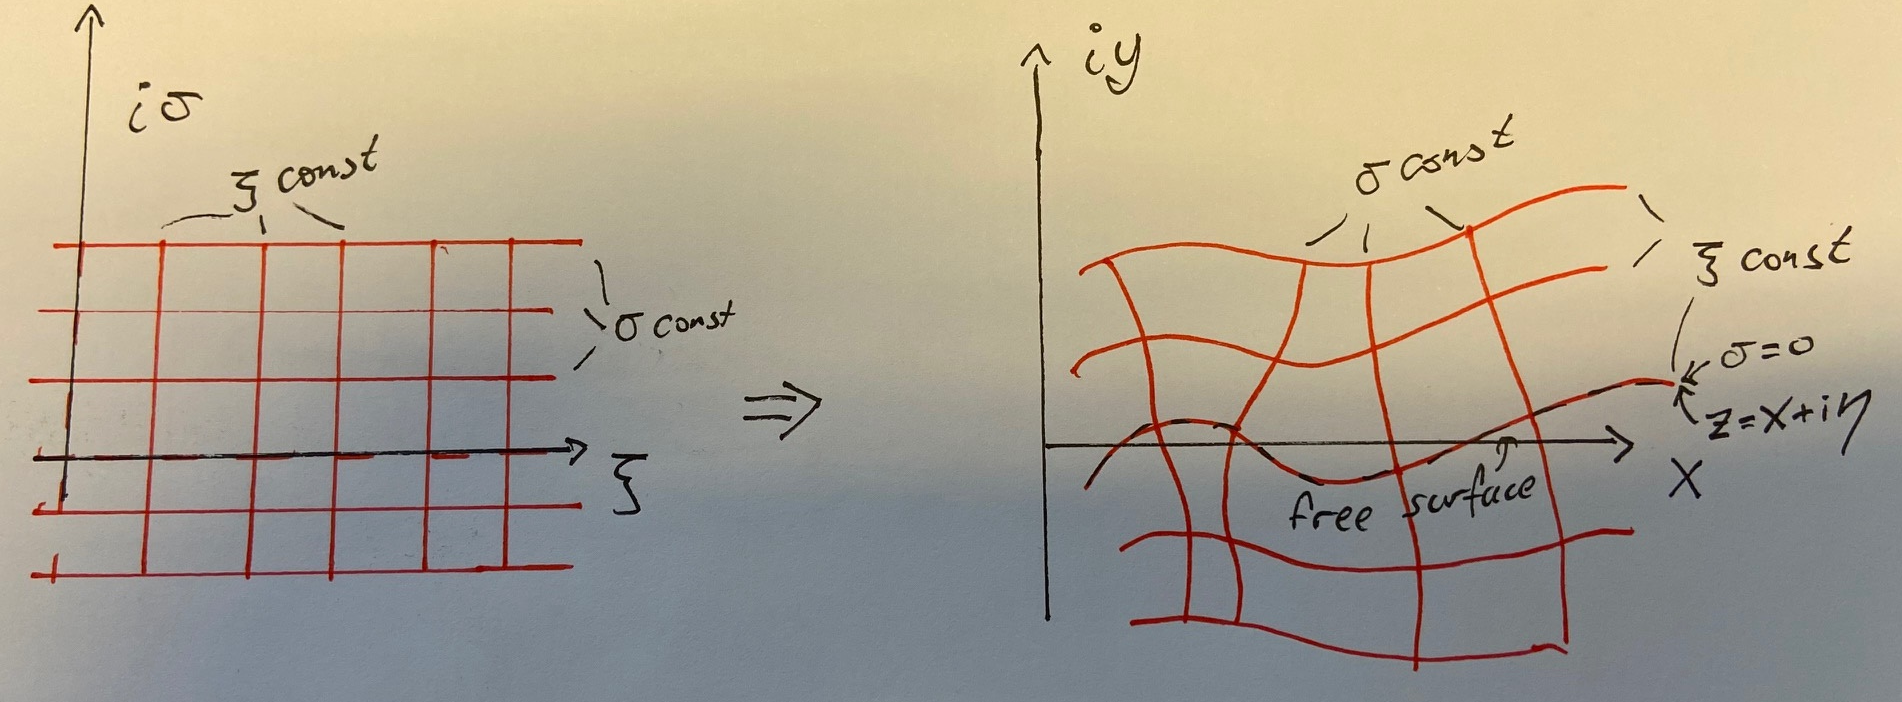
\includegraphics[width=.75\columnwidth]{./figures/map.png}%
\caption{Conformal map, mapping line $\yy=0$ to the free surface $\y=\surf$.}%
\label{fig:map}%
\end{figure}
\begin{figure}[h!ptb]%
\centering
\includegraphics[width=.75\columnwidth]{./conformal.pdf}%
\caption{The map \eqref{eq:map} in the physical $\z$-plane when $\eta(\x)$ is a single harmonic of wavenumber $\pi/2$ and amplitude $0.1$.}%
\label{fig:mapReg}%
\end{figure}

The aim of this mapping is to allow for evaluation of potential function gradients at the free surface. 
To this endeavour, we project a complex potential filed from the rectangular $\zz$-plane onto the physical $\z$-plane,
\begin{equation}
%\w(\z) = \ww[\zz(\z)],
\w(\z) = \ww[\zzmap(\z)].
\label{eq:wProj}
\end{equation}
A complex potential is defined
\[ \ww(\zz) = \phi(\xx,\yy) + \ii \psi(\xx,\yy), \]
$\phi$ being the potential function and $\psi$ the stream function in the rectangular plane.
%We have available the free surface values of the potential function $\phi\S(x)$ and so the function matching is
We have available the potential $\phi\S(\x)$ at the free surface of the physical $\z$-plane, which constitutes the line $\yy=0$ in the rectangular  $\zz$-plane. 
Accordingly, we match the functions
\begin{equation}
%\Re \w(x+\ii\surf) = \Re \ww(x) = \phi\S(x).
\phi\S(\x) = \Re \w(\x+\ii\surf) = \Re \ww[\zzmap(\x+\ii\surf)] = \Re \ww(\x).
\label{eq:wMatch}
\end{equation}
Equations \eqref{eq:invMap} and \eqref{eq:wProj} were here invoked to demonstrate the matching.
The deep water
%\footnote{In intermediate depth $h$, $\ww(\zz) = \sum_{j=0}^\infty a_j \frac{\sin k_j(\zz+\ii h)}{\cosh k_j h}$.}
 complex potential is  in the rectangular plane defined as a combination of positive wavenumber Fourier modes
\begin{equation}
\ww(\zz) = \sum_{j=0}^\infty \h\ww_j \ee^{\ii k_j \zz}; \quad k_j\geq 0.
\label{eq:w}
\end{equation}
Matching condition \eqref{eq:wMatch} yields
\begin{equation}
\h\ww_0 = \h\phi_0\S, \quad \h\ww_j = 2\big(\h\phi\S_j\big)^*;\; j>0, 
\label{eq:aj}
\end{equation}
$\{\h\phi\S_j\}$ being the Fourier components of $\phi\S(x)$ and asterisk denoting the complex conjugate.

We now have the ingredients necessary to compute the velocities $U=u+\ii v$ at the free surface. 
The chain rule yields
\begin{equation*}
%U^* = \dd{\w}{\z}\bigg|_{0} = \dd{}{\z}\ww[\zz(\z)]\bigg|_0 = \dd\ww\zz\dd\zz\z\bigg|_0 = \bigg(\dd\ww\zz\bigg|_0\bigg)\bigg(\dd\z\zz\bigg|_0\bigg)^{-1},
U_0^* = \dd{\w}{\z}\bigg|_{0} = \dd{}{\z}\ww[\zzmap(\z)]\bigg|_0 = \ww'/\zmap' \big|_0,
%\label{eq:U_derive}
\end{equation*}
zero denoting evaluation at surface $\z=\x+\ii\surf$, $\zz=\xx$.
Inserting \eqref{eq:map} and \eqref{eq:w}, the full expression becomes
\begin{equation}
U^*(\x+\ii\surf) = \frac{1}{\ii- \surf_{\x}}\sum_{j=0}^\infty  k_j \h\ww_j \ee^{-\ii k_j \x},
\label{eq:U}
\end{equation}
with, of course, $\surf_\x=\sum_{j=-\infty}^\infty\ii k_j\h\surf_j\ee^{\ii k_j \x}$.
\\

We remark on the unexpected explicitness of this approach. 
Conformal mapping strategies often require inverse mapping $\zzmap$ which cannot be preformed explicitly. 
A key feature of the problem at hand is however that we only require potential function \textit{derivatives} along a prescribed path.






\section{The conformal mapping technique in finite water depth}
\label{sec:H}
Unsurprisingly, the conformal map suggested in equation \eqref{eq:map} turns out not to be original, with similar mappings fond in e.g.~\citet{chalikov2005modeling}, although its usefulness in deep-water application in the context described above appears to be unremarked.
The deep water assumption may at first glance may look like a minor simplification, but it is in fact essential for the explicitness and simplicity of the above scheme. 
Let's look at the problems faced by a finite depth.
\\

The conformal map, equivalent to \eqref{eq:map}, with a finite water depth $H$ is
\begin{equation}
z\mapsto \zmap(\zz) = \zz - \ii \sum_{j=-\infty}^\infty \h\eta_j \frac{\ee^{\ii k_j(\zz+\ii H)}}{\sinh kH}.
\label{eq:map_H}
\end{equation}
This map does \textit{not} have the property \eqref{eq:mapXi} but rather
\begin{equation}
\Im \zmap(\xx) = \surf(\xx).
\label{eq:ImMapXi}
\end{equation}
The difference is that $\zmap(\xx)$ comes with a stretching of the $x$-dimension where
\begin{equation}
\Re \zmap(\xx) \equiv x\S(\xx) = \xx -\ii  \sum_{j=-\infty}^\infty \h\eta_j \frac{\ee^{\ii k_j\xx}}{\tanh kH}
\label{eq:mapXi}
\end{equation}
(the latter term also being real).
This means that $\surf(\xx)$ in \eqref{eq:ImMapXi}, the surface boundary in the $\zz$-plane, is no functionally equivalent to the the surface $h(\x)$ in the physical plane, but rather
$\eta(\xx)=h[x\S(\xx)]$, and it is the Fourier components of $\eta(\xx)$, not of $h(\x)$, that are required in \eqref{eq:map_H}.
In other words, the mapping \eqref{eq:map_H} is highly implicit in both directions.
It is easily plotted reversely---given a function $\eta$ in the $\zz$-plane we can compute the map \eqref{eq:map_H} and see what physical surface $h(x)$ this corresponds to.
An example is shown in \autoref{fig:map_H} for a sinusoidal $\eta(\xx)$. Note that the surface $h(x)$ in the physical plane is not sinusoidal.

Other parts of the scheme would be fairly similar; we have $\zzmap[x\S(\xx)+\ii\eta(\xx)]=\xx$, etc.
The complex potential of finite depth is in the $\zz$-plane is
\begin{equation}
%\ww(\zz) = \sum_{j=0}^\infty\h\ww_j \frac{\sin k_j(\zz+\ii H)}{\cosh k_j H}; \quad \h\ww_j\in\mathbb R,\; k_j\geq 0.
\ww(\zz) = \sum_{j=-\infty}^\infty\h\ww_j \frac{\ee^{\ii k_j(\zz+\ii H)}}{\cosh k_j H}; \quad \h\ww_{-j}=\h\ww_{j}^*.
\label{eq:wH}
\end{equation}
The stretching $x\S(\xx)$ further affects the mapping of $\phi\S(\x)$ into the coefficients $\{\h\ww_j\}$.

\begin{figure}[h!ptb]%
\centering
\includegraphics[width=.75\columnwidth]{./conformalH.pdf}%
\caption{The map \eqref{eq:map_H} in the physical $\z$-plane when $\eta(\xx)$ is a single harmonic of wavenumber $\pi$ and amplitude $0.075$. $H=0.75$.}%
\label{fig:map_H}%
\end{figure}




\section{Conformal mapping to emulate the presence to steep alterations in bathymetry}

Assume we have mapped a flat-bedded domain in the $\zz$-plane into a curvilinear $\z$ plane. 
A common example such a mapping is the Schwarz--Christoffel  transformation $\z\mapsto \zmap(\zz)$ with
\[
\zmap'(\zz) = C \prod_{j=1}^J (\zz-\xx_j)^{-\alpha_j/\pi},
\]
in which the horizontal coordinate is bent stiff angles $\alpha_j$ at locations $\zeta=\xi_j$.
Some particular mappings are analytically integrable, such as the orthogonal step which yields
\begin{equation}
\zmap(\zz) = \frac {H\_d-H\_s}\pi \left[  \sqrt{\zz-1}\sqrt{\zz+1} - 2\sinh^{-1}\! \sqrt{(\zz-1)/2} \right] - \ii H\_s,
\label{eq:SC}
\end{equation}
$H\_d$ and $H\_s$ being the deep and shallow sides of the step, respectively.%
\footnote{This is mapping the plane into $\zz_1=-1$, $\zz_2=1$. A less streched map is obtained if mapping into, say, $\zz_1=-d$, $\zz_2=0$; $d=H\_d-H\_s$, yielding
\[
\zmap(\zz) =   \frac {2d}\pi \left[  \sqrt{\zz/d}\sqrt{\zz/d+1} - \log\left(\sqrt{\zz/d} \sqrt{\zz/d+1}\right) \right] - \ii H\_s,
\]
 }
Map \eqref{eq:SC} cannot be analytically inverted.

The complex potential with an impermeable surface at $\yy=0$ is
\begin{equation}
\ww(\zz) = \sum_{j=-\infty}^\infty\h\ww_j \ee^{\ii k_j\zz}; \quad \h\ww_{-j}=\h\ww_{j}^*.
\label{eq:w0}
\end{equation}

It is impractical in practice to map a transient free surface within a simulation routine, as noted in \autoref{sec:H}.
We can however map $\zz$ to the reference plane $\y = 0$ which is fixed throughout the simulation, and from there use the traditional HOS technique of Taylor expansion.
Let's call such a mapping $\zz_0(\x)$. It satisfies
\[
\z[\zz_0(x)]=x.%\in\mathbb R.
\]
Such a map is easily computed numerically using interpolation; the circles in \autoref{fig:SC_step} shows $\z[\zz_0(x)]$ for regularly spaced $x$.
\\

\begin{figure}[h!ptb]%
\centering
\subfloat[$\z$-plane]{\includegraphics[width=.5\columnwidth]{../conformalMapping/SC_step.pdf}}%
\subfloat[$\zz$-plane]{\includegraphics[width=.5\columnwidth]{../conformalMapping/SC_step_inv.pdf}}%
\caption{A step mapped with the Schwarz--Christoffel transform \eqref{eq:SC}}%
\label{fig:SC_step}%
\end{figure}


Next we consider the Taylor expansion routine from which the vertical velocity at the free surface is to be determined. 
This procedure inverts the expansion 
\[
\phi\S = \phi(x,h(x)) = \sum_{m=0}^\infty \frac{h^m}{m!}\partial_y^m \phi(x,0)
\]
combined with the order expansion 
\begin{equation}
\phi=\sum_{n=1}^N\phi\oo n
\label{eq:phiExpansion}
\end{equation}
to get
\begin{equation}
\phi\oo{n}(x,0) = 
\begin{cases}
\phi\S(x), & n = 1,\\
- \sum_{m=1}^{n-1} \frac{h^m}{m!}\partial_y^m \phi\oo{n-m}(x,0), & n>1.
\end{cases}
\label{eq:phioon}
\end{equation}
In terms of the complex potential $\w\oo n(\z)=\phi\oo n(\x,\y)+\ii \psi\oo n(\x,\y)$ we have 
\begin{equation}
\partial_y^m \phi\oo{n} = \Re\left\{ \mr{d}_\z^n\w(\z) \ee^{\ii \frac\pi2 n} \right\} .
\label{eq:ppphi}
\end{equation}
It is straightforward to related the derivatives of $\w(\z)$ to the derivatives of $\ww(\zz)$ in \eqref{eq:w0} using the derivatives of \eqref{eq:SC} and the chain rule. 


\section{Conformal step with flat surface $y=0$}
The step map displayed in \autoref{fig:map_H} can be given a flat surface $y=0$ with some added complexity in the transformation function.
We base such a map on the common presented task of finding a flow field over a step in a channel \citep[e.g.,][\SSS 4.3.2]{mei_2005}.
The complex potential there created can itself be regarded as a conformal map.
Accordingly, we have
\begin{subequations}
\begin{align}
\lambda &= \exp(\zeta + \ii \pi),\label{eq:map_Hflat:lambda}\\
%t &= \frac{^+\!\sqrt{\lambda-c^2}}{^+\!\sqrt{\lambda-1}},\label{eq:map_Hflat:t}\\
t &= \sqrt{\frac{\lambda-c^2}{\lambda-1} },\label{eq:map_Hflat:t}\\
z &\mapsto f(\zeta) = -\ii H\_s +\frac{H\_d}{\pi}\left[ 
\frac1c \ln^+\frac{t-c}{t+c} - \ln\frac{t-1}{t+1}
\right]\label{eq:map_Hflat:z},
\end{align}%
\label{eq:map_Hflat}%
\end{subequations}%
with $c = H\_d/H\_s$.
The map \eqref{eq:map_Hflat} goes via the map \eqref{eq:map_Hflat:lambda}, mapping $\zeta$ the polar plane $\lambda$ (normally considered a stream function source), and the right angled $t$-plane \eqref{eq:map_Hflat:t}.
The flat-surface domain of $z=\x+\ii\y$, $\y\leq0$ is mapped by the strip $\zz=\xx+\ii\yy$, $-\pi<\yy\leq0$.
With waves present it may be necessary to evaluate $\z$ at locations $\y>0$; $\yy>0$ for which care must be taken on order to choose the appropriate branches of the square roots and logarithms. 
%Accordingly, we have in \eqref{eq:map_Hflat} introduced in the operators $^+\!\sqrt{\phantom{\cdot} }$ and $\ln^+$, the angles of which run from $0$ to $\pi$ and $0$ to $2\pi$, respectively.  
Accordingly, we have in \eqref{eq:map_Hflat:z} introduced in the operator $\ln^+$, the angles of which run from $0$ to $2\pi$. 
\autoref{fig:Mei_step} shows the adjusted map \eqref{eq:map_Hflat} for $-\pi\leq\yy\leq0.5$ with the intermediate planes $\lambda(\zz)$ and $t(\lambda)$ shown in \autoref{fig:Mei_step_lambda_t}.
Note that the free surface $\y=0$ is a straight line  $\yy=0$ in the $\zz$-plane, but that $\xx$ is contracted over the step transition.
The direction of the step is reversed by flipping the abscissa; $z\mapsto-f(-\zeta)$.  
\begin{figure}[h!ptb]%
\centering
\subfloat[$\z$-plane]{\includegraphics[width=.5\columnwidth]{../conformalMapping/CCMei_step.pdf}}%
\subfloat[$\zz$-plane]{\includegraphics[width=.5\columnwidth]{../conformalMapping/CCMei_step_inv.pdf}}%
\caption{A step mapped with adjusted Schwarz--Christoffel transform \eqref{eq:map_Hflat}}%
\label{fig:Mei_step}%
\end{figure}

\begin{figure}[h!ptb]%
\centering
\subfloat[$\lambda(\zz)$-plane]{\includegraphics[width=.37\columnwidth]{../conformalMapping/CCMei_step_lambda.pdf}}%
\qquad
\subfloat[$t(\lambda)$-plane]{\includegraphics[width=.5\columnwidth]{../conformalMapping/CCMei_step_t.pdf}}%
\caption{The intermediate maps \eqref{eq:map_Hflat:lambda} and \eqref{eq:map_Hflat:t}}%
\label{fig:Mei_step_lambda_t}%
\end{figure}

\bibliographystyle{plainnat} % abbrvnat,plainnat,unsrtnat
\bibliography{bib,sintef_bib} %You need a file 'literature.bib' for this.


\end{document}
